\documentclass[10pt]{beamer}

%%%
% PREAMBLE FOR THIS DOC 
%%%
%https://tex.stackexchange.com/questions/68821/is-it-possible-to-create-a-latex-preamble-header
\usepackage{/Users/miw267/Repos/csci246_spring2025/slides/preambles/beamer_preamble_for_CSCI246}



%%% TRY TO RESHOW TOC AT EACH SECTION START (with current section highlighted)
% Reference: https://tex.stackexchange.com/questions/280436/how-to-highlight-a-specific-section-in-beamer-toc
\newcommand\tocforsect[2]{%
  \begingroup
  \edef\safesection{\thesection}
  \setcounter{section}{#1}
  \tableofcontents[#2,currentsection]
  \setcounter{section}{\safesection}
  \endgroup
}


%%%% HERES HOW TO DO IT CORRECTLY
% FIRST IN .STY FILE, DO
%\usetheme[sectionpage=none]{metropolis}
% THEN AT EACH SECTION DO
%\begin{frame}{Outline}
%  \tableofcontents[currentsection]	
%\end{frame}



%\setbeamertemplate{navigation symbols}{}
%\setbeamertemplate{footline}[frame number]{}


%%%
% DOCUMENT
%%%

\begin{document}

%\maketitle

%% Title page frame
%\begin{frame}
%    \titlepage 
%\end{frame}





\title{02/24/2025: Relations}
\author{CSCI 246: Discrete Structures}
\date{Textbook reference: Sec 14, Scheinerman}

\begin{frame}
    \titlepage 
\end{frame}


\begin{frame}
\footnotesize 
\begin{mygreenbox}[title=Graded Quiz Pickup]
Quizzes are in the front of the room, grouped into four bins (A-G, H-L, M-R, S-Z) by last name. The quizzes are upside down with your last name on the back. Come find yours before, during, or after class.  Only turn the quiz over if it's yours.
\end{mygreenbox} 
\vfill 

\begin{myredbox}[title=Announcements]

\begin{itemize}
\item Regrades from last Friday (2/14) are available.  
\end{itemize}

\end{myredbox}

\vfill 


\begin{myyellowbox}[title=Today's Agenda]
\begin{itemize}
	\item Reading quiz (5 mins)
	\item Mini-lecture ($\approx$ 10 mins)
%	%
%	\begin{itemize}
%	\footnotesize 
%	\item Review induction 
%	\end{itemize}
%	%
	\item Group exercises ($\approx$ 30 mins)
\end{itemize}

%	Rationale for group exercises: we got shortchanged on time last couple days, and I already did a lot of lectures, so I want you to practice. Next problems quiz will cover relations and functions: Hamkins and 
%	
\end{myyellowbox}
\vfill 

\end{frame}

\begin{frame}
 \begin{myredbox}[title=Reading Quiz (Relations)]    
 For each of the following relations defined on the integers, please state whether the relation is reflexive, symmetric, and/or transitive.
 
 \begin{enumerate}
 	\item $=$ (equality)
 	\item $\leq$ (less than or equal to)
 	\item $<$ (strict less than)
 	\item $|$ (divides)
 \end{enumerate}

\end{myredbox}
	
\end{frame}


\begin{frame}[standout]
Feedback on Friday's Quiz	
\end{frame}

\begin{frame}{Scores On Problems Quiz (Quantifiers and Set Operations)}
\footnotesize 
\begin{figure}[ht]
        \centering
        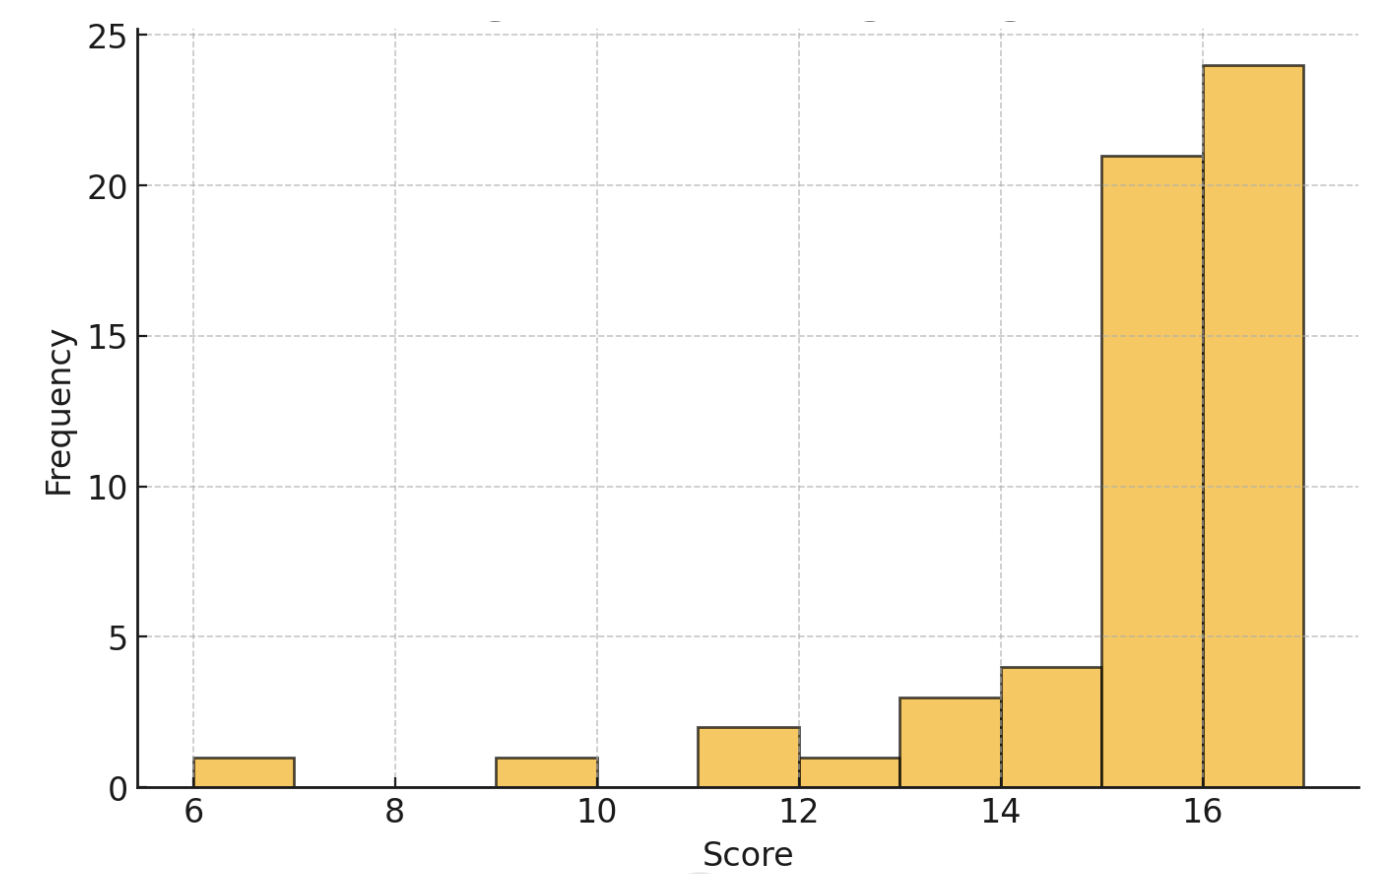
\includegraphics[width=.75\textwidth]{images/problems_quiz_scores}
   		 \caption{Median Score = 15/16 (93.7\%)}
\end{figure}
\vfill 
\textbf{Rubric.} 

\begin{enumerate}
	\item Quantifiers question (8 points total): 1 point for each subquestion (a)-(h)
	\item Set operations question (8 points total): 4 points for the correct answer. 4 points for a correct explanation.
\end{enumerate}




\end{frame}

\begin{frame}{Scores On Reading Quiz (Intro to Functions) (Extra Credit)}
\footnotesize 
\begin{figure}[ht]
        \centering
        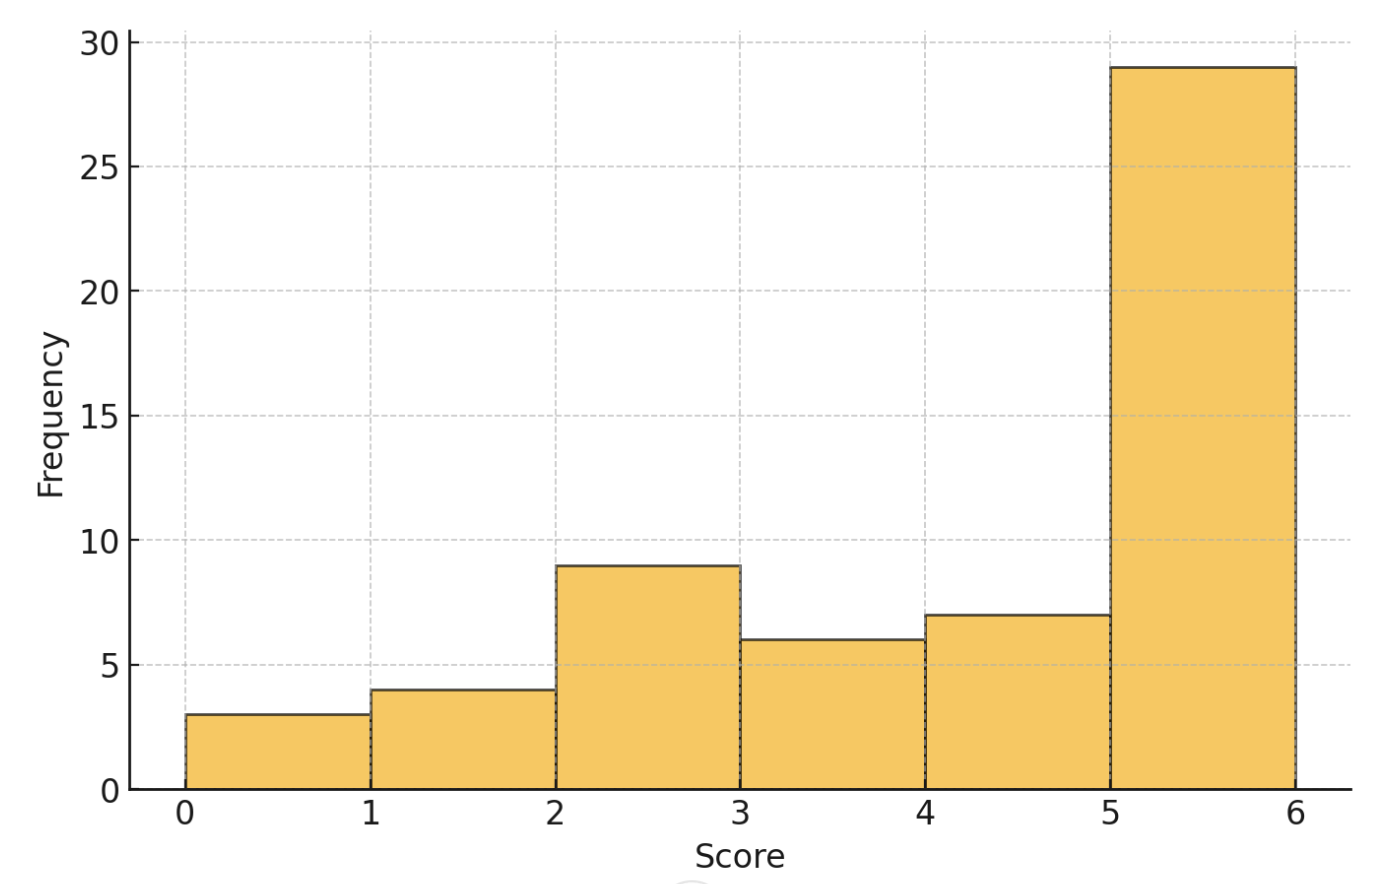
\includegraphics[width=.75\textwidth]{images/reading_quiz_scores}
   		 \caption{Median Score = 4.5/5 (90\%)}
\end{figure}
\vfill 
\textbf{Rubric.}  1 point for each diagram if correct.

\end{frame}


\begin{frame}[standout]
High-level re-motivation
\end{frame}


\begin{frame}{Cybersecurity}
\footnotesize 
\begin{figure}[ht]
        \centering
        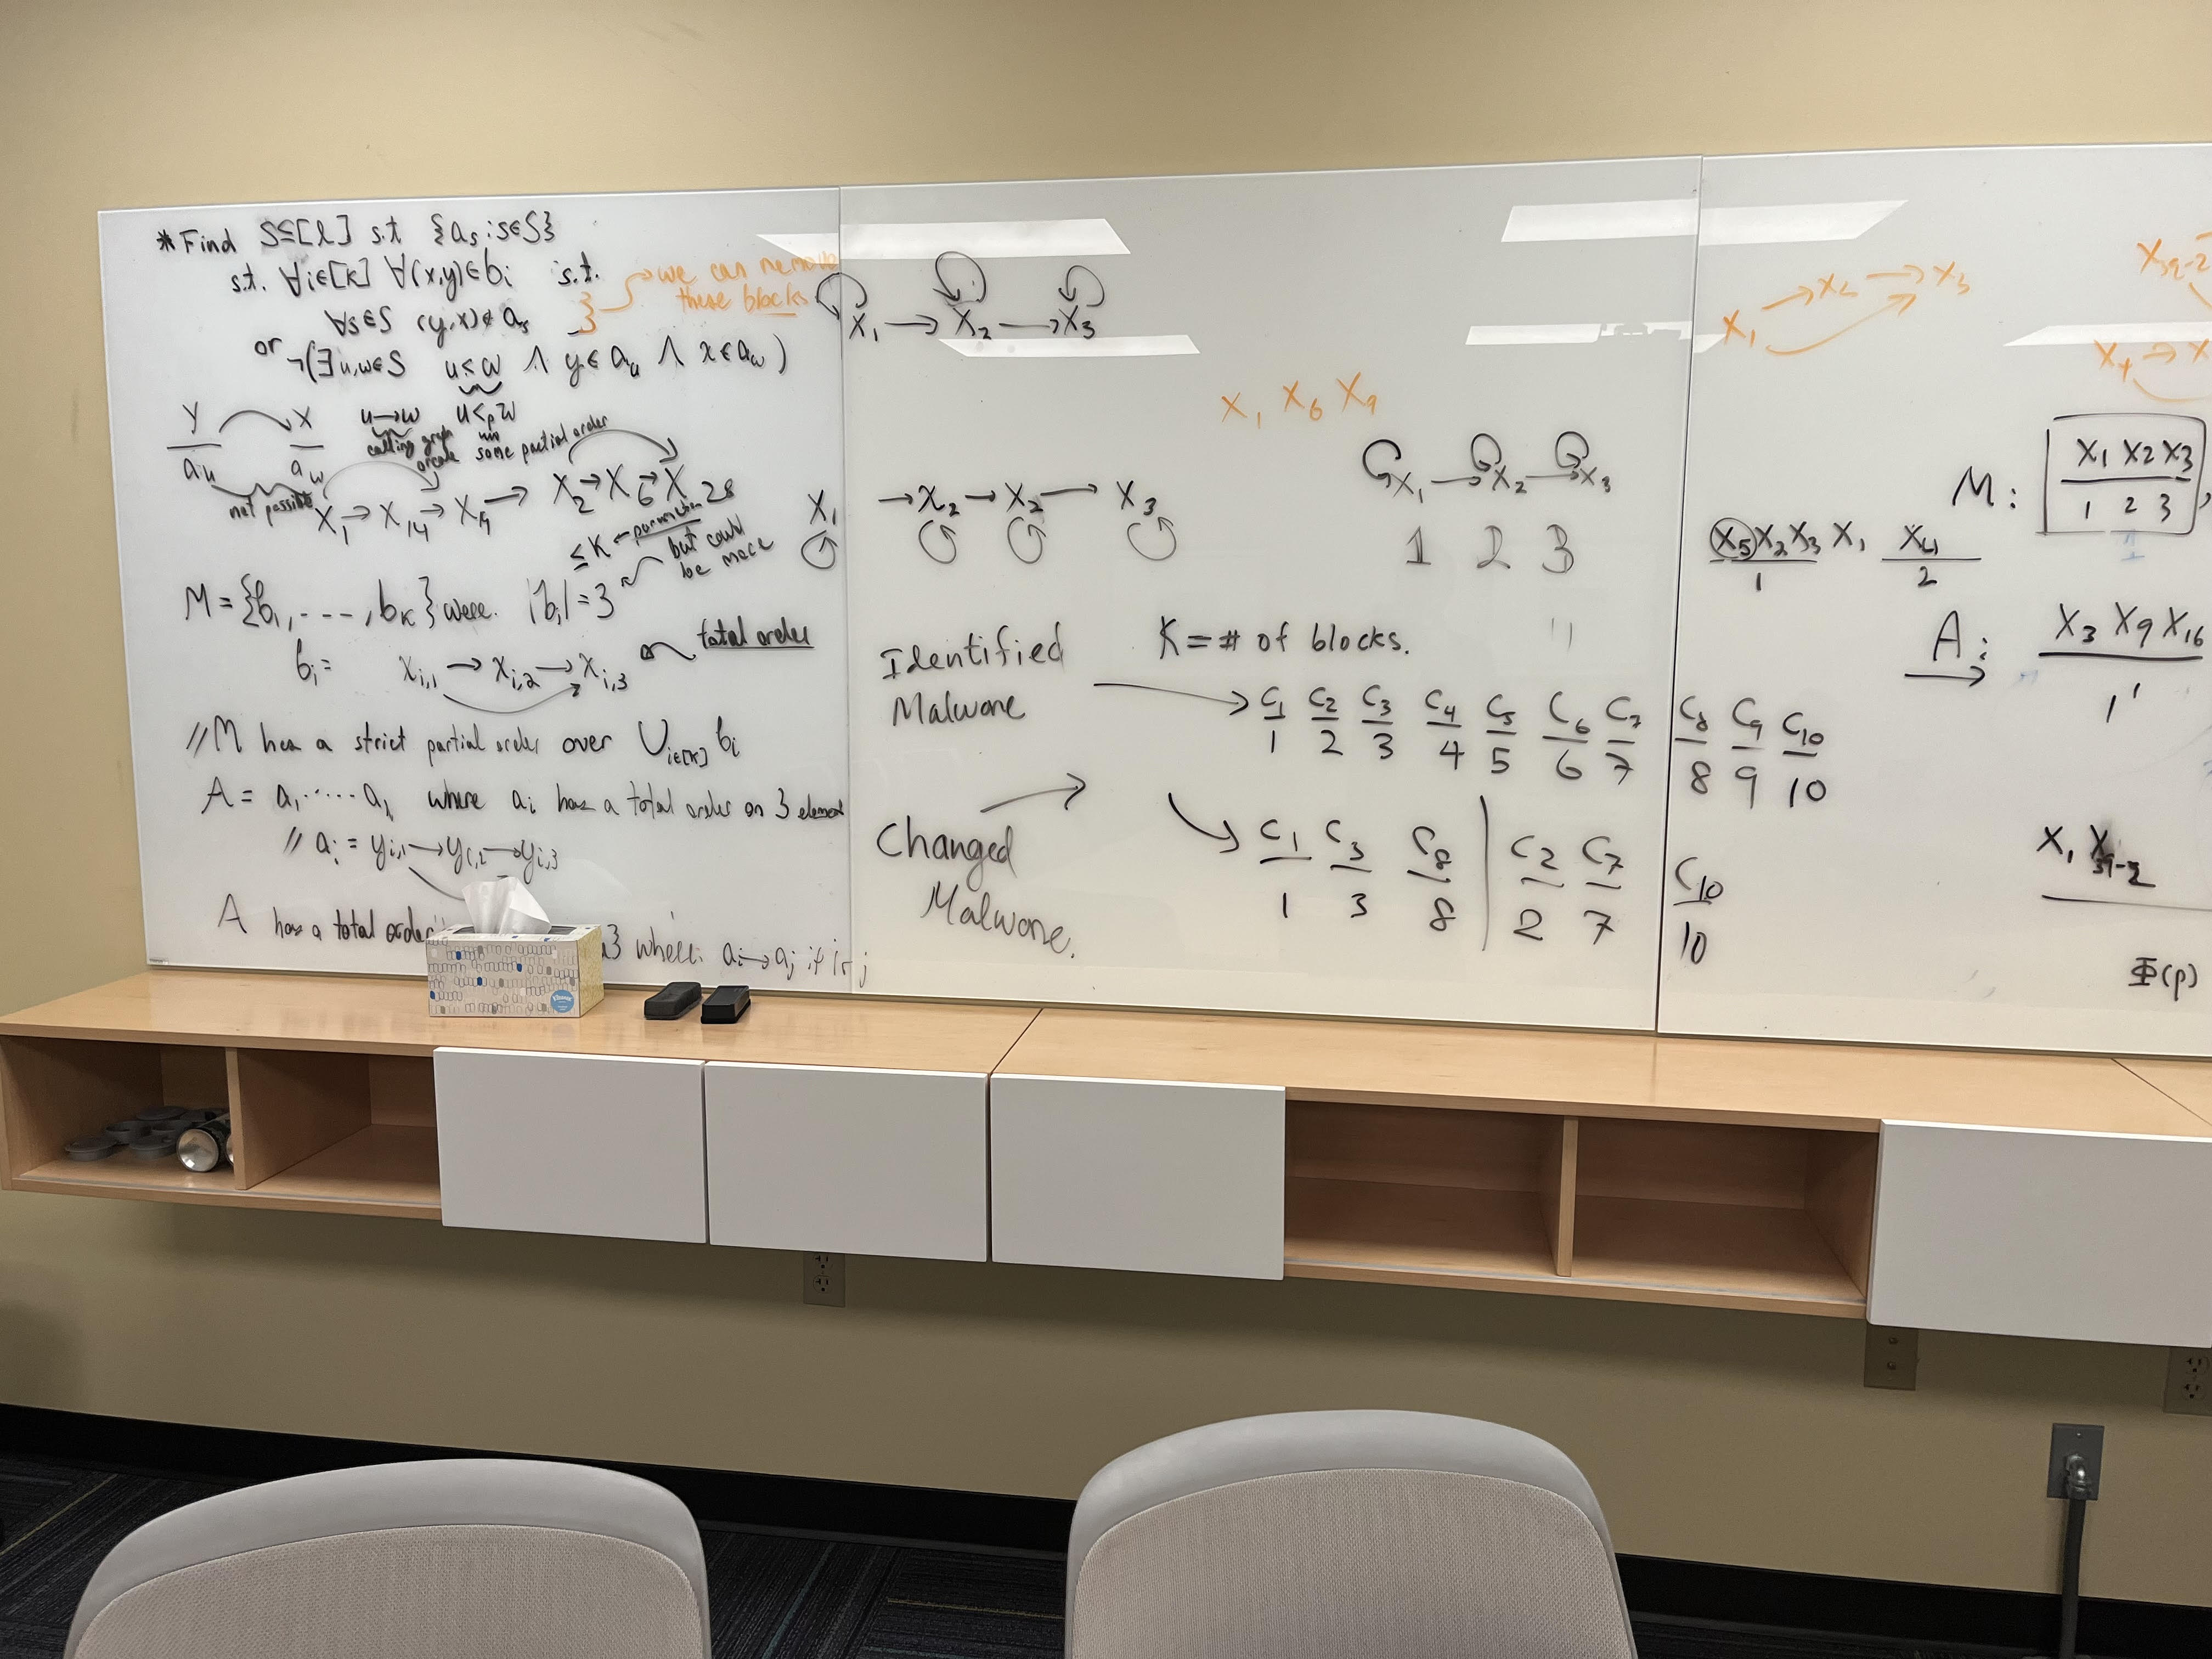
\includegraphics[width=.8\textwidth]{images/cyber}
   		 %\caption{Median Score = 4.5/5 (90\%)}
   		 
   		 \begin{textblock*}{-3cm}(11cm,7cm)  % (x-position, y-position), with the width of the image
        
\includegraphics[width=2cm]{images/fangtian_zhong.jpg}  % Change image name and size as needed
    \end{textblock*}
    
\end{figure}
\end{frame}

\begin{frame}{Machine Learning}
\footnotesize 
\begin{figure}[ht]
        \centering
        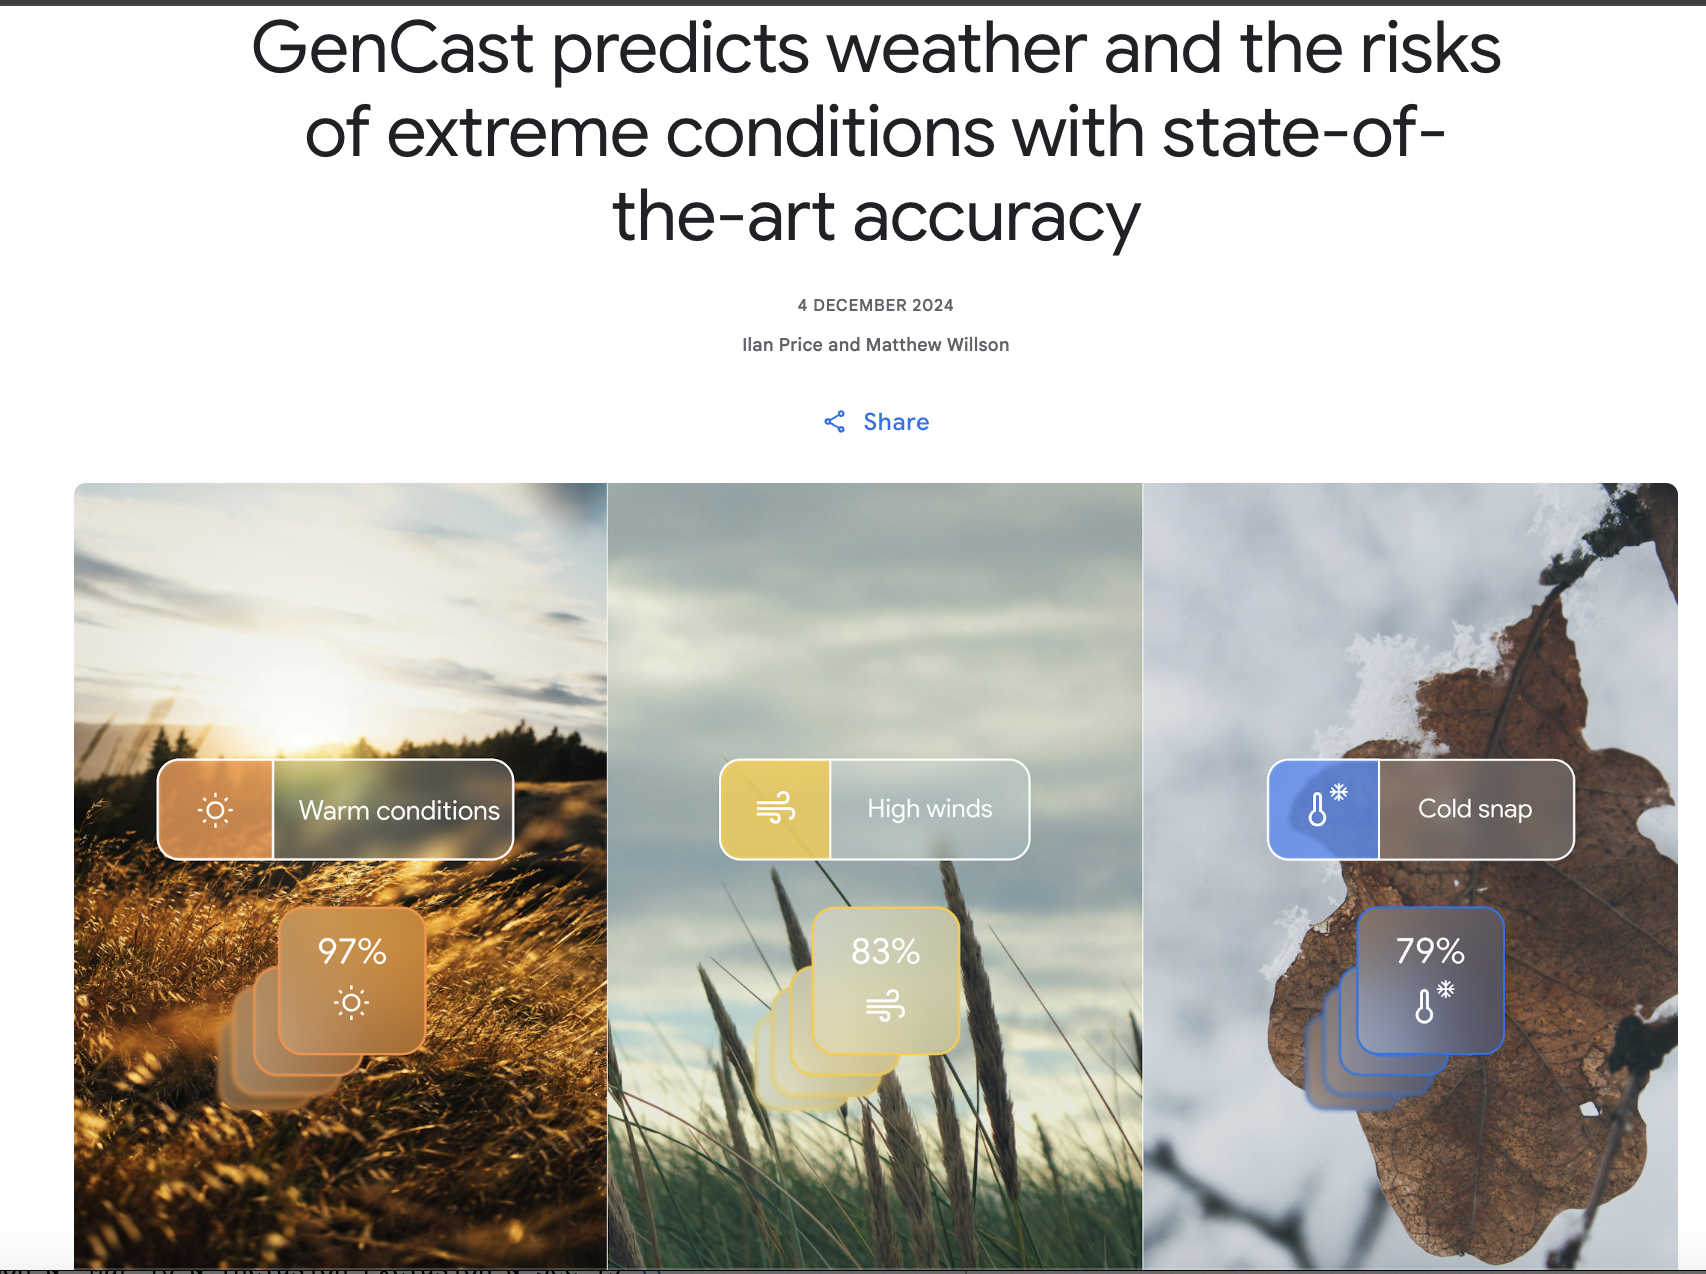
\includegraphics[width=\textwidth]{images/gencast_0}
   		 %\caption{Median Score = 4.5/5 (90\%)}
\end{figure}
\end{frame}



\begin{frame}{Machine Learning}
\footnotesize 
\begin{figure}[ht]
        \centering
        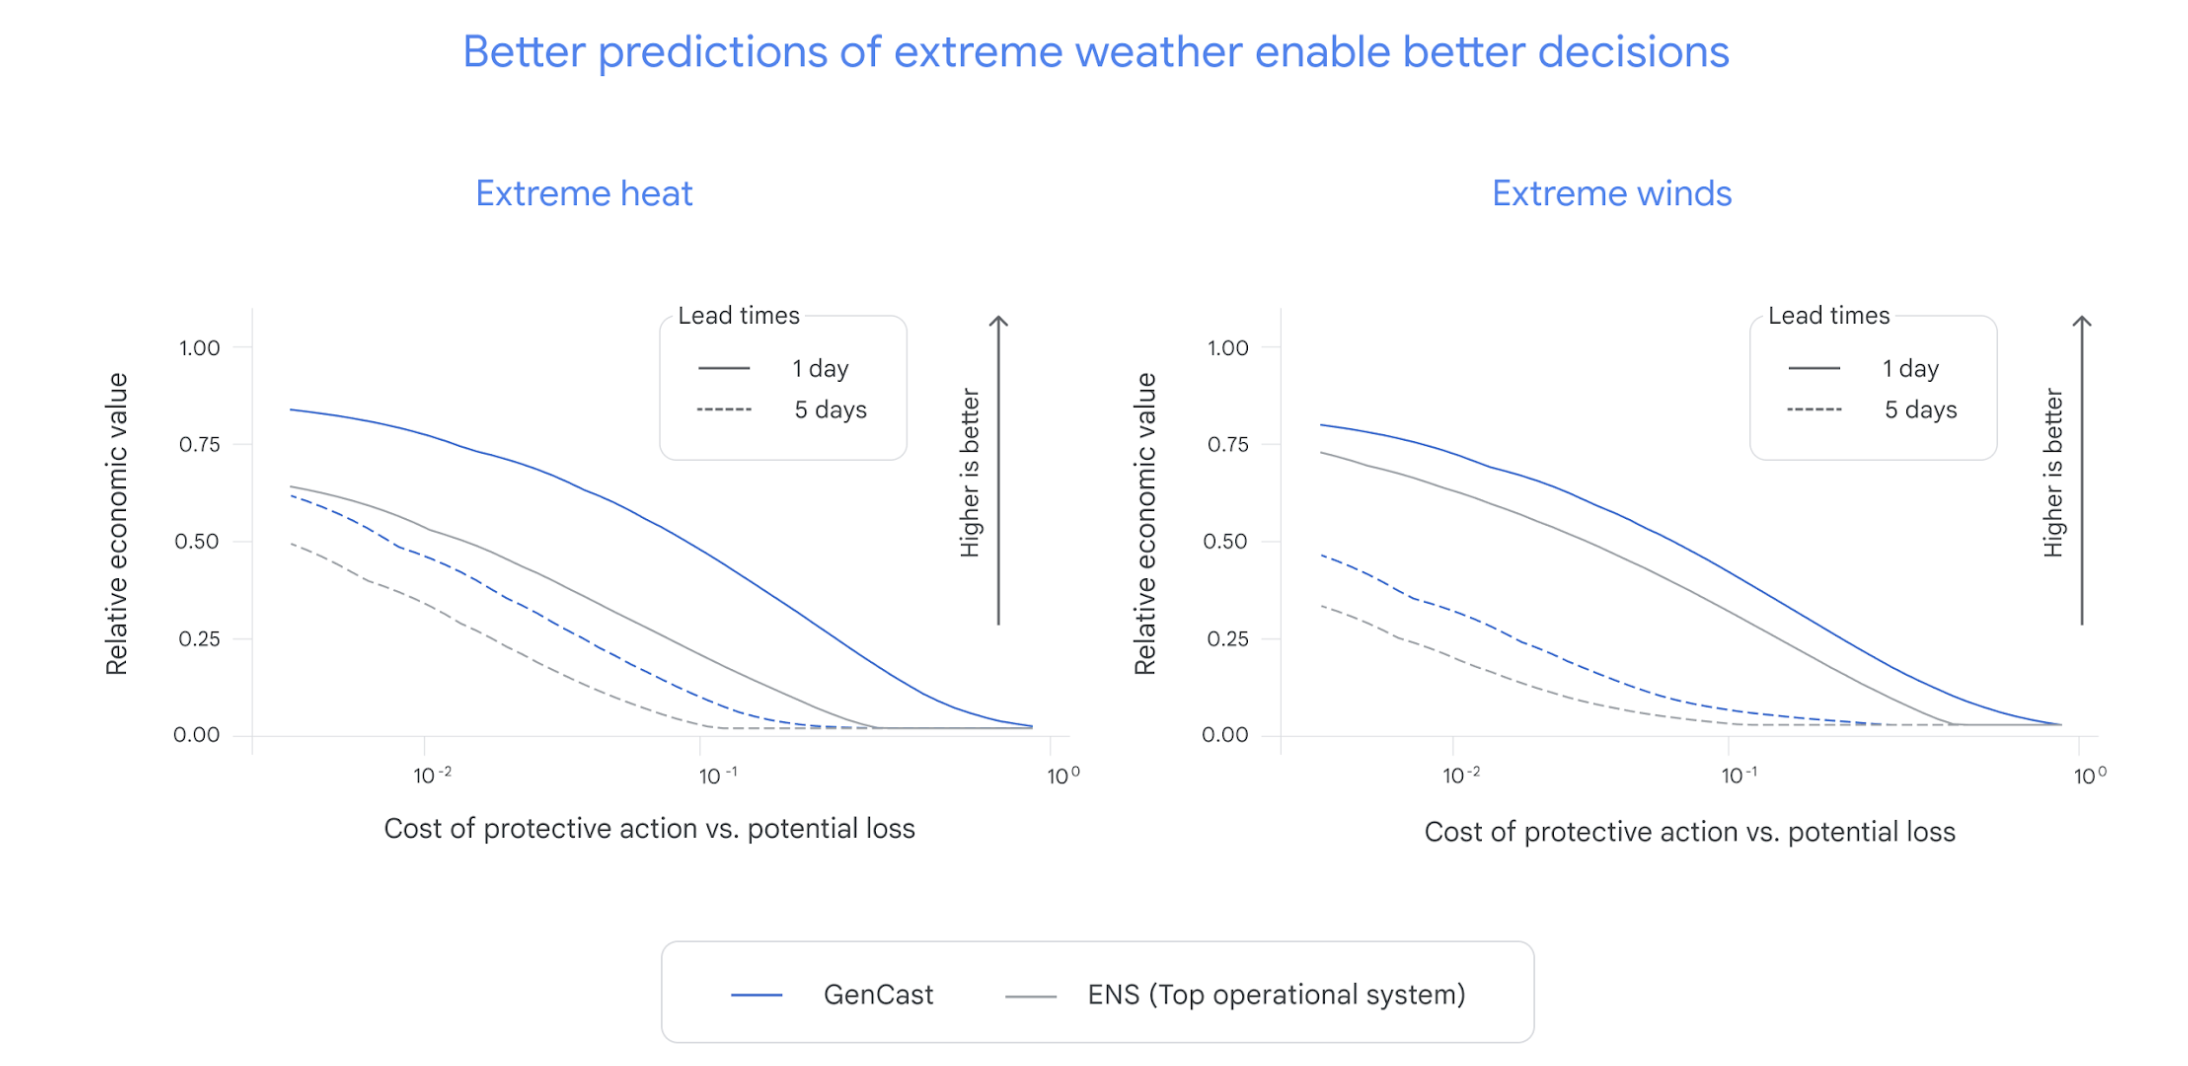
\includegraphics[width=\textwidth]{images/gencast_1}
   		 %\caption{Median Score = 4.5/5 (90\%)}
\end{figure}
\end{frame}


\begin{frame}{Machine Learning}
\footnotesize 
\begin{figure}[ht]
        \centering
        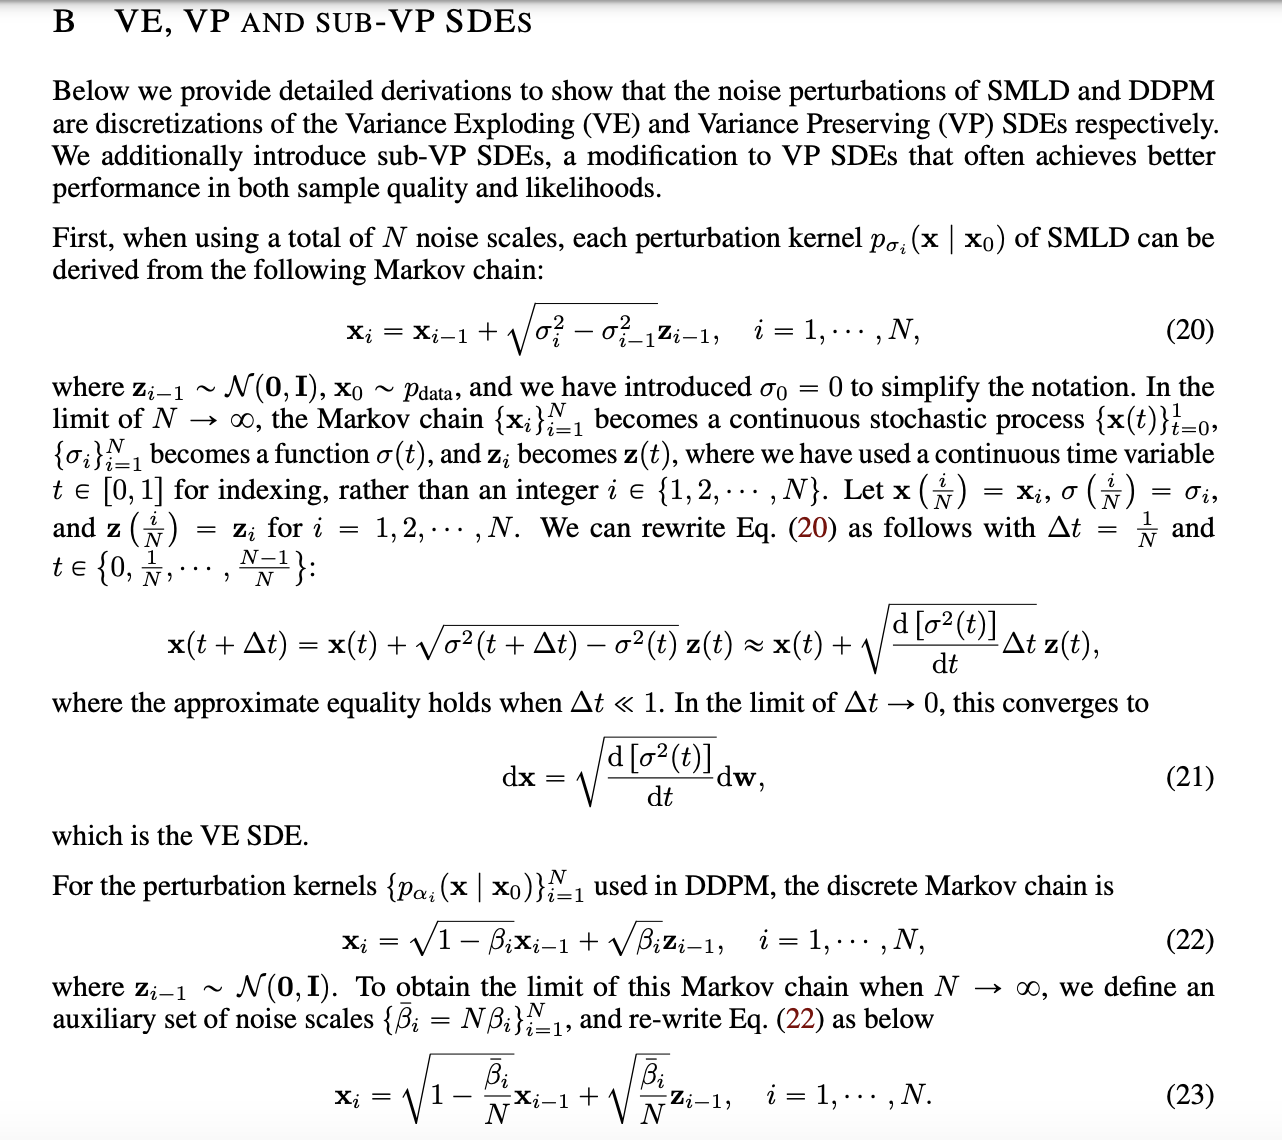
\includegraphics[width=.8\textwidth]{images/gencast_3}
   		 %\caption{Median Score = 4.5/5 (90\%)}
\end{figure}
\end{frame}

\begin{frame}{Machine Learning}
\footnotesize 
\begin{figure}[ht]
        \centering
        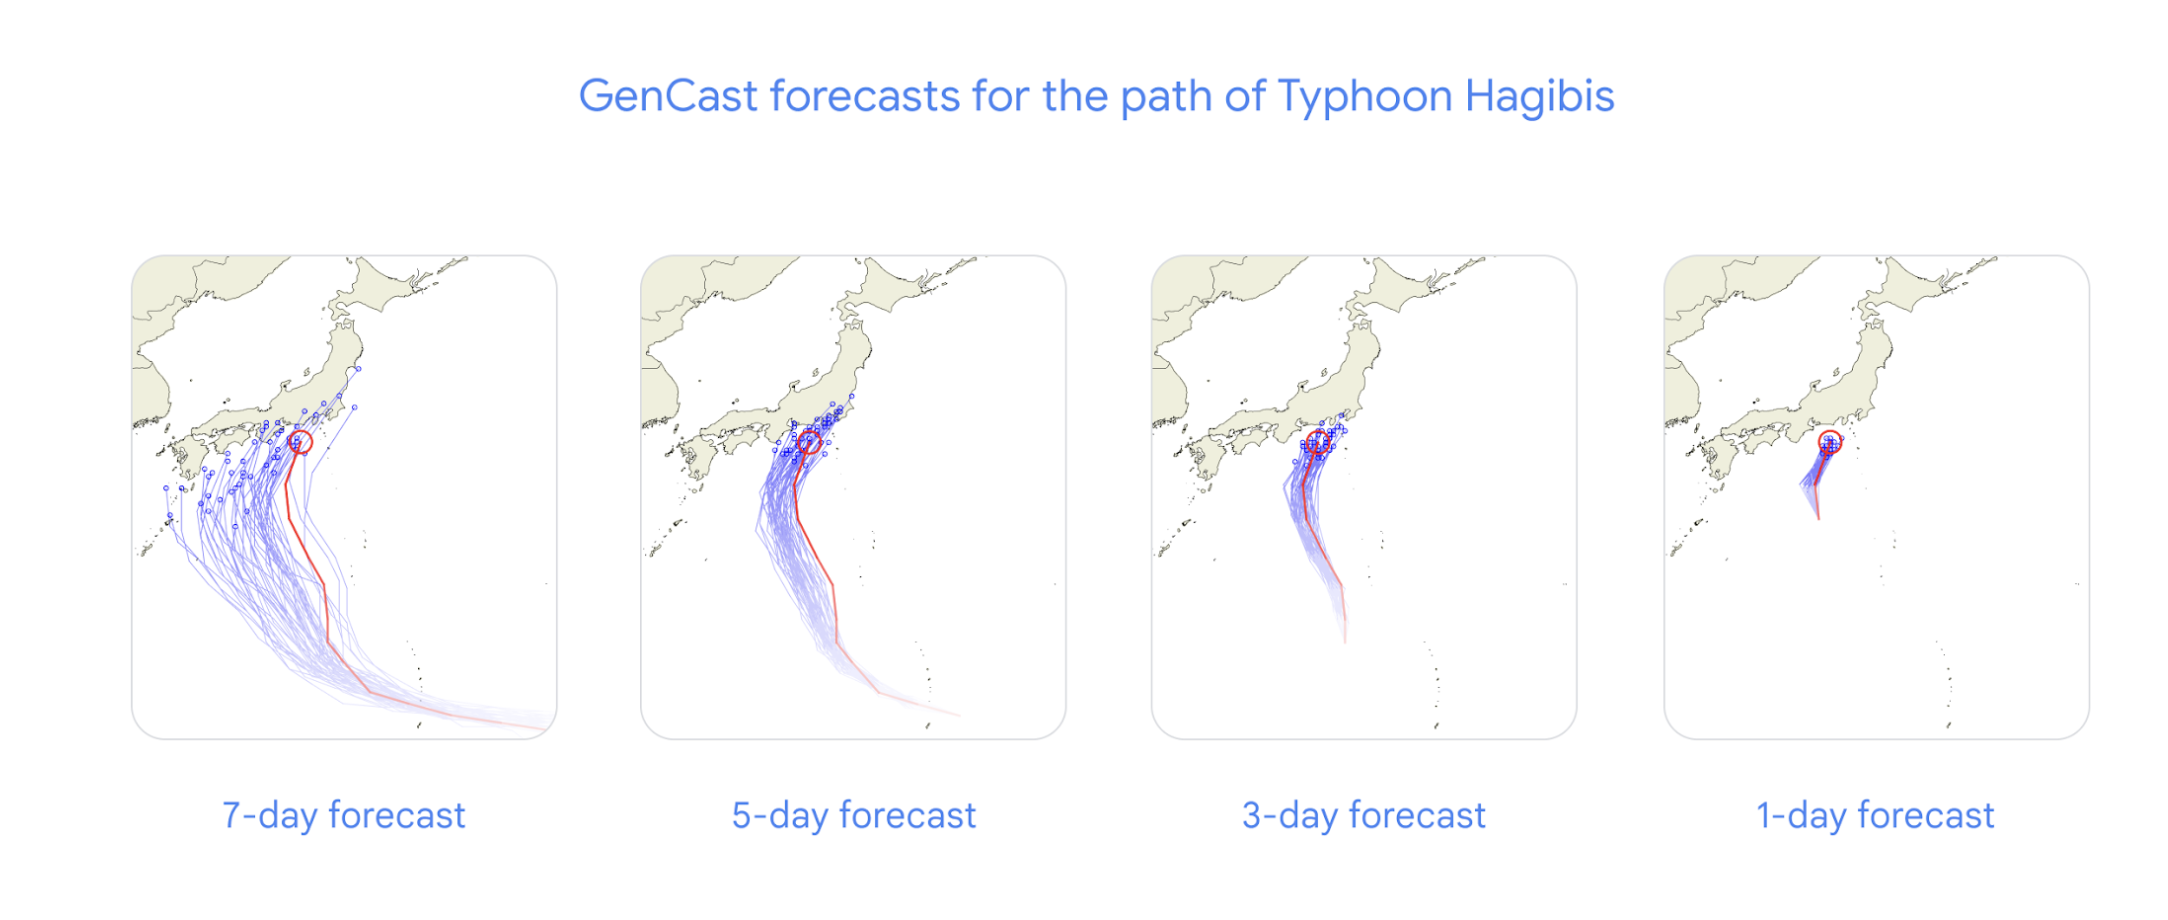
\includegraphics[width=\textwidth]{images/gencast_2}
   		 %\caption{Median Score = 4.5/5 (90\%)}
\end{figure}
\end{frame}


\begin{frame}[standout]
Drawing pictures of relations
\end{frame}


\begin{frame}

\begin{myredbox}[title=Drawing relations from $A$ to $B$]
 To draw a picture of relation $R$ from $A$ to $B$, we draw two collections of dots. The first collection of dots corresponds to elements in $A$, and we place these on the left side of the figure. The dots for $B$ go on the right. We then draw an arrow from $a \in A$ to $b \in B$ just when $(a,b)$ is in the relation.  
 \end{myredbox}
 
\begin{mygreenbox}[title=Example]
Let $A = \set{1,2,3,4,5}$ and $B=\set{4,5,6,7}$, and let $R$ be the relation $\set{(1,4),(1,5),(2,5),(3,6)}$.  A picture of the relation $R$ is given in the figure below.  
 
 \begin{figure}
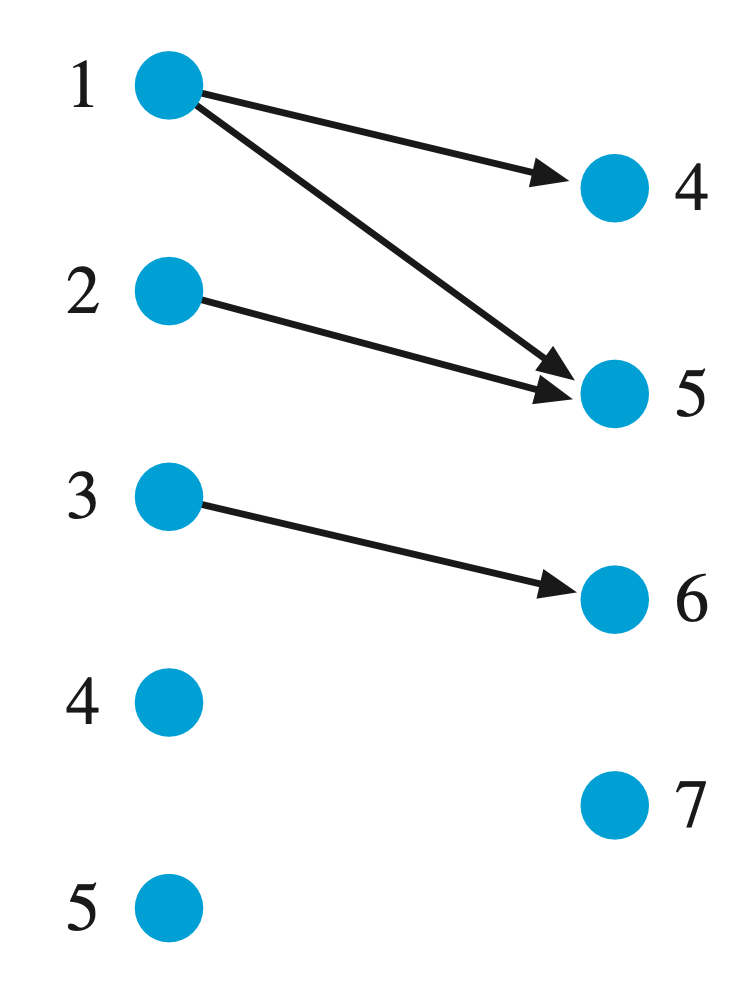
\includegraphics[width=.2\textwidth]{images/relations} 
\end{figure}

\end{mygreenbox}
 


\end{frame}


\begin{frame}

\begin{myredbox}[title=Drawing relations on $A$]
 To draw a picture of relation $R$ on $A$, we have two options
 \begin{enumerate}
  	\item We can make a diagram in which each element of $A$ is represented by a dot.  If $aRb$, then we draw an arrow from dot $a$ to dot $b$.  If it happens that $b$ is also related to $a$, then we draw another arrow from $b$ to $a$. If $aRa$, then we draw a looping arrow form $a$ to itself.
 	\item We can consider this as a relation $R$ from $A$ to $A$, and use the method of the previous slide.
 \end{enumerate}
 \end{myredbox}
 
\begin{mygreenbox}[title=Example]
Let $A = \set{1,2,3,4,5}$ and $R=\set{(1,1), (1,2), (1,3), (4,3), (3,1)}$. A picture of the relation $R$ (using option \#1) is given in the figure below.  
 
 \begin{figure}
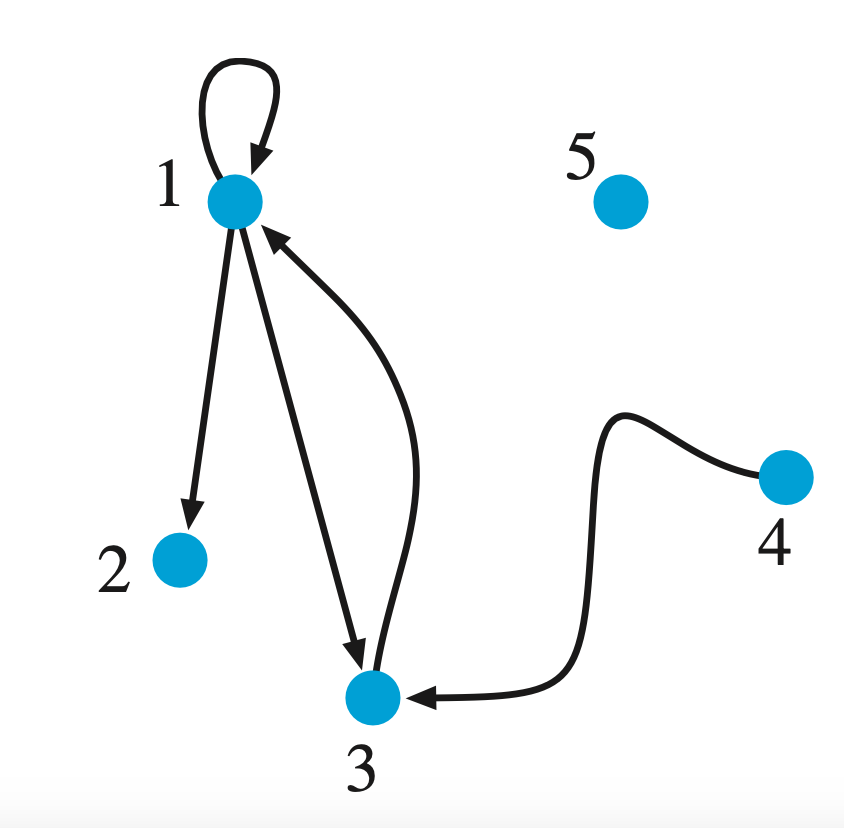
\includegraphics[width=.2\textwidth]{images/relations_on_A} 
\end{figure}

\end{mygreenbox}
 


\end{frame}



\begin{frame}

\begin{mygreenbox}[title=An Example Using a Set with Infinitely Many Elements]
Let $A = \mathbb{Z}$ and $R$ be the $\leq$ relation.  A picture of the relation is given below 
 \begin{figure}
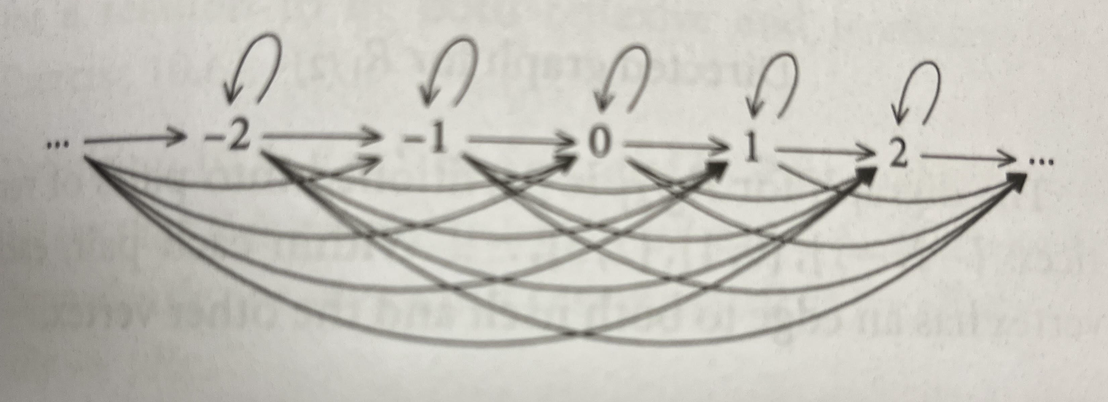
\includegraphics[width=\textwidth]{images/leq} 
\end{figure}

\end{mygreenbox}
 


\end{frame}



\begin{frame}[standout]
Group exercises
\end{frame}

\begin{frame}
\footnotesize 
\vfill 
\begin{columns}
\begin{column}{0.33\textwidth}
aaron.loomis: 3 \\ 
adam.wyszynski: 13 \\ 
alexander.goetz: 21 \\ 
alexander.knutson: 9 \\ 
anthony.mann: 19 \\ 
blake.leone: 1 \\ 
bridger.voss: 12 \\ 
caitlin.hermanson: 11 \\ 
cameron.wittrock: 14 \\ 
carsten.brooks: 6 \\ 
carver.wambold: 1 \\ 
colter.huber: 0 \\ 
conner.reed1: 16 \\ 
connor.graville: 20 \\ 
connor.mizner: 3 \\ 
connor.yetter: 15 \\ 
delaney.rubb: 4 \\ 
derek.price4: 7 \\ 
devon.maurer: 20 \\ 
emmeri.grooms: 21 \\ 
erik.moore3: 8 \\ 
ethan.johnson18: 15 \\\end{column}
\begin{column}{0.33\textwidth}
evan.barth: 14 \\ 
evan.schoening: 13 \\ 
griffin.short: 11 \\ 
jack.fry: 7 \\ 
jacob.ketola: 13 \\ 
jacob.ruiz1: 2 \\ 
jacob.shepherd1: 0 \\ 
jada.zorn: 16 \\ 
jakob.kominsky: 3 \\ 
james.brubaker: 8 \\ 
jeremiah.mackey: 10 \\ 
jett.girard: 19 \\ 
john.fotheringham: 20 \\ 
jonas.zeiler: 0 \\ 
joseph.mergenthaler: 15 \\ 
joseph.triem: 2 \\ 
julia.larsen: 7 \\ 
justice.mosso: 8 \\ 
kaden.price: 16 \\ 
lucas.jones6: 12 \\ 
luka.derry: 11 \\ 
luke.donaldson1: 1 \\\end{column}
\begin{column}{0.33\textwidth}
lynsey.read: 5 \\ 
mason.barnocky: 17 \\ 
matthew.nagel: 9 \\ 
micaylyn.parker: 4 \\ 
michael.oswald: 9 \\ 
nolan.scott1: 14 \\ 
owen.obrien: 19 \\ 
pendleton.johnston: 6 \\ 
peter.buckley1: 18 \\ 
peyton.trigg: 17 \\ 
reid.pickert: 12 \\ 
ryan.barrett2: 2 \\ 
samuel.hemmen: 6 \\ 
samuel.mosier: 5 \\ 
samuel.rollins: 21 \\ 
sarah.periolat: 5 \\ 
timothy.true: 4 \\ 
tristan.nogacki: 17 \\ 
tyler.broesel: 10 \\ 
william.elder1: 18 \\ 
yebin.wallace: 10 \\ 
zeke.baumann: 18 \\\end{column}
\end{columns}
	
\end{frame}




\begin{frame}{Group Exercises: Relations}
\footnotesize 
\begin{enumerate}
	\item \textit{(Relations as ordered pairs.)}  Write the following relations on the set $\set{1,2,3,4,5}$ as sets of ordered pairs: (a) is-less-than, (b) is-divisible-by, (c) is-equal-to, (d) has-the-same-parity-as.  (Note: When we say two numbers have the same parity, we mean they are both odd or both even.)
\item \textit{(Drawing pictures of relations.)} 
	Draw pictures of the following relations on $A$. 
	\begin{itemize} \footnotesize 
		\item[a.] Let $A=\set{a \in \mathbb{N} : a|10}$ and let $R$ be the relation $|$ (divides) restricted to $A$. 
		\item[b.] Let $A=\set{1,2,3,4,5}$ and let $R$ be the relation  $=$ (equals) restricted to $A$.
	\end{itemize}
\item \textit{(Drawing pictures of relations.)}  Draw pictures of the following relations on $A \times B$.
	\begin{itemize} \footnotesize 
		 \item[a.] Let $A=\set{1,2,3,4}$ and $B = \set{2,3,4}$. Let $R$ be the relation $\geq$ (greater than or equal to) from $A$ to $B$.
	\end{itemize}

	\item \textit{(Properties of relations.)} The property \textit{irreflexive} is not the same as being not reflexive.  To illustrate this, do the following: (a) Give an example of a relation on a set that is neither reflexive nor irreflexive.  (b) Give an example of a relation on a set that is both reflexive and irreflexive.  
	Part (a) is not too hard, but for (b), you will need to create a rather strange example.
	
	\item \textit{(Properties of relations.)} For each of the following relations on the set of all human beings, determine whether the relation is reflexive, irreflexive, symmetric, anti-symmetric, and/or transitive: (a) is-taller-than, (b) has-the-same-parents-as (i.e., same mother and father), (c)  is-the-child-of, (d) is-married-to.


\end{enumerate}
\end{frame}

\begin{frame}{Solution to Group Exercise \#1}
\footnotesize 
\textbf{Problem.} \textit{(Relations as ordered pairs.)}  Write the following relations on the set $\set{1,2,3,4,5}$ as sets of ordered pairs: (a) is-less-than, (b) is-divisible-by, (c) is-equal-to, (d) has-the-same-parity-as.  (Note: When we say two numbers have the same parity, we mean they are both odd or both even.)
\vfill 
\textbf{Solution.}
\begin{itemize}
\item[a.]
\[ \begin{array}{cccc}
R= & \bigg\{ & (1,2), (1,3), (1,4), (1,5), & \\
  & & (2,3), (2,4), (2,5),  &\\
   & & (3,4), (3,5), (4,5)  & \bigg\} \\
\end{array} \]    

\item[b.]
\[ R= \bigg\{  (1,1), (2,1), (3,1), (4,1), (5,1),(2,2), (4,2)  \bigg\} \]
\item[c.]
\[ R= \bigg\{  (1,1), (2,2), (3,3), (4,4), (5,5)  \bigg\} \]
\item[d.]
\[ \begin{array}{cccc}
R= & \bigg\{ & (1,1), (1,3), (1,5), (3,1), (3,3), (3,5), (5,1), (5,3), (5,5), & \\
   & & (2,2), (2,4), (4,4), (4,2)  & \bigg\} \\
\end{array} \]  
\end{itemize}
\end{frame}

\begin{frame}{Solution to Group Exercise \#2a}
\textbf{Problem.} \textit{(Drawing pictures of relations.)} 
	Draw pictures of the following relation on $A$: Let $A=\set{a \in \mathbb{N} : a|10}$ and let $R$ be the relation $|$ (divides) restricted to $A$. 
\vfill 
\textbf{Solution.} First note that $A=\set{1,2,5,10}$.  Now we draw

\begin{center}
\begin{tikzpicture}

% Nodes in a vertical line
\node[latent] (1) at (0, 3) {1};
\node[latent] (2) at (0, 2) {2};
\node[latent] (5) at (0, 1) {5};
\node[latent] (10) at (0, 0) {10};

% Curved edges
\path[->, >=stealth, bend left=60] (1) edge (2);
\path[->, >=stealth, bend left=60] (1) edge (5);
\path[->, >=stealth, bend left=60] (1) edge (10);
\path[->, >=stealth, bend left=60] (2) edge (10);
\path[->, >=stealth, bend left=60] (5) edge (10);

% Self loops
\path[->, >=stealth, loop left] (1) edge (1);
\path[->, >=stealth, loop left] (2) edge (2);
\path[->, >=stealth, loop left] (5) edge (5);
\path[->, >=stealth, loop left] (10) edge (10);
\end{tikzpicture}
\end{center}

\end{frame}


\begin{frame}{Solution to Group Exercise \#2b} 
\textbf{Problem.} \textit{(Drawing pictures of relations.)} 
	Draw pictures of the following relation on $A$: Let $A=\set{1,2,3,4,5}$ and let $R$ be the relation  $=$ (equals) restricted to $A$.
	
\vfill 
\textbf{Solution.} We draw 

\begin{center}
\begin{tikzpicture}

% Nodes in a vertical line
\node[latent] (1) at (0, 4) {1};
\node[latent] (2) at (0, 3) {2};
\node[latent] (3) at (0, 2) {3};
\node[latent] (4) at (0, 1) {4};
\node[latent] (5) at (0, 0) {5};


% Self loops
\path[->, >=stealth, loop left] (1) edge (1);
\path[->, >=stealth, loop left] (2) edge (2);
\path[->, >=stealth, loop left] (3) edge (3);
\path[->, >=stealth, loop left] (4) edge (4);
\path[->, >=stealth, loop left] (5) edge (5);
\end{tikzpicture}
\end{center}

\end{frame}

\begin{frame}{Solution to Group Exercise \#3}
\textbf{Problem.} \textit{(Drawing pictures of relations.)} 
	Draw pictures of the following relations on $A \times B$: Let $A=\set{1,2,3,4}$ and $B = \set{2,3,4}$. Let $R$ be the relation $\geq$ (greater than or equal to) from $A$ to $B$.

	
\vfill 
\textbf{Solution.} We draw 

\begin{center}
\begin{tikzpicture}

% Nodes in a vertical line
\node[latent] (A1) at (-2, 3) {1};
\node[latent] (A2) at (-2, 2) {2};
\node[latent] (A3) at (-2, 1) {3};
\node[latent] (A4) at (-2, 0) {4};
\node[latent] (B2) at (1, 2) {2};
\node[latent] (B3) at (1, 1) {3};
\node[latent] (B4) at (1, 0) {4};


% Edges
\path[->, >=stealth] (A2) edge (B2);
\path[->, >=stealth] (A3) edge (B2);
\path[->, >=stealth] (A3) edge (B3);
\path[->, >=stealth] (A4) edge (B2);
\path[->, >=stealth] (A4) edge (B3);
\path[->, >=stealth] (A4) edge (B4);
\end{tikzpicture}
\end{center}

\end{frame}


\begin{frame}{Solution to Group Exercise \#4a}
\footnotesize 
\textbf{Problem.} \textit{(Properties of relations.)} 
The property \textit{irreflexive} is not the same as being not reflexive.  To illustrate this, do the following: (a) Give an example of a relation on a set that is neither reflexive nor irreflexive.  (b) Give an example of a relation on a set that is both reflexive and irreflexive.  
	Part (a) is not too hard, but for (b), you will need to create a rather strange example.
	
\vfill 
\textbf{Solution to (a).}  The solution is determined by the red loops below.

\begin{table}[H]
\centering 	
\begin{tabular}{ccc}
\textbf{Reflexive} & \textbf{Irreflexive} & \textbf{Neither} \\
$xRx \; \forall \; x \in A$	& $x\cancel{R}x \; \forall \; x \in A$	&\\
\begin{tikzpicture}

% Nodes in a vertical line
\node[latent] (1) at (0, 4) {a};
\node[latent] (2) at (0, 3) {b};
\node[latent] (3) at (0, 2) {c};
\node[latent] (4) at (0, 1) {d};


% Self loops
\path[->, >=stealth, loop left, red] (1) edge (1);
\path[->, >=stealth, loop left, red] (2) edge (2);
\path[->, >=stealth, loop left, red] (3) edge (3);
\path[->, >=stealth, loop left, red] (4) edge (4);

% Curved edges
\path[->, >=stealth, bend left=60] (1) edge (2);
\path[->, >=stealth, bend left=60] (1) edge (4);
\path[->, >=stealth, bend left=60] (2) edge (4);
\end{tikzpicture} 
& 
\begin{tikzpicture}

% Nodes in a vertical line
\node[latent] (1) at (0, 4) {a};
\node[latent] (2) at (0, 3) {b};
\node[latent] (3) at (0, 2) {c};
\node[latent] (4) at (0, 1) {d};

% Curved edges
\path[->, >=stealth, bend left=60] (1) edge (2);
\path[->, >=stealth, bend left=60] (1) edge (4);
\path[->, >=stealth, bend left=60] (2) edge (4);
\end{tikzpicture} 
& 

\begin{tikzpicture}

% Nodes in a vertical line
\node[latent] (1) at (0, 4) {1};
\node[latent] (2) at (0, 3) {2};
\node[latent] (3) at (0, 2) {3};
\node[latent] (4) at (0, 1) {4};


% Self loops
\path[->, >=stealth, loop left, red] (1) edge (1);
%\path[->, >=stealth, loop left, red] (2) edge (2);
%\path[->, >=stealth, loop left, red] (3) edge (3);
\path[->, >=stealth, loop left, red] (4) edge (4);

% Curved edges
\path[->, >=stealth, bend left=60] (1) edge (2);
\path[->, >=stealth, bend left=60] (1) edge (4);
\path[->, >=stealth, bend left=60] (2) edge (4);
\end{tikzpicture}
\end{tabular}
\end{table}

%\vfill 
%\textbf{Solution to (b).}  Let $R$ be any relation on the empty set $\emptyset$.  Then both conditions hold vacuously.  (Recall the truth table for implication.)
\end{frame}


\begin{frame}{Solution to Group Exercise \#4b}
\footnotesize  
\textbf{Problem.} \textit{(Properties of relations.)} 
The property \textit{irreflexive} is not the same as being not reflexive.  [...] Give an example of a relation on a set that is both reflexive and irreflexive.  
\vfill 

\textbf{Solution to (b).}  Let $R$ be any relation on the empty set $\emptyset$.  Then the conditions of reflexive and irreflexive both hold vacuously. If this seems puzzling, let's recall the truth table for implication.  

\vfill 
\begin{table}
\centering
\begin{tabular}{cc|c}
\multicolumn{2}{c}{\textbf{Original propositions}} & \textbf{New proposition} \\
P & Q & $P \implies Q$ \\
\hline 
T & T & \green{T} \\
T & F & \red{F}  \\
F & T & \green{T}  \\
F & F & \green{T} \\
\end{tabular}
\end{table}

 We can write the condition for reflexivity as
 \[ \explaintermbrace{P}{x \in A} \; \implies \; \explaintermbrace{Q}{aRa}\]
and the condition for irreflexivity as
\[ \explaintermbrace{P}{x \in A} \; \implies \; \explaintermbrace{Q}{a\cancel{R}a}\] 
In other words, the hypothesis $P$ is always false, so the statements are tautologies.
\end{frame}


\begin{frame}{Solution to Group Exercise \#5}
\textbf{Problem.} \textit{(Properties of relations.)} 
For each of the following relations on the set of all human beings, determine whether the relation is reflexive, irreflexive, symmetric, anti-symmetric, and/or transitive: (a) is-taller-than, (b) has-the-same-parents-as (i.e., same mother and father), (c)  is-the-child-of, (d) is-married-to.
	
\vfill 
\textbf{Solution.} 

\begin{itemize}
\item[a.] Irreflexive, anti-symmetric (vacuously), transitive.
\item[b.] Reflexive, symmetric, transitive.
\item[c.] Irreflexive, anti-symmetric (vacuously)
\item[d.] Irreflexive, symmetric, transitive (vacuously).
\end{itemize}

\end{frame}


\end{document}
